\documentclass{standalone}
\usepackage{tikz}
\usetikzlibrary{automata,positioning}

\begin{document}
  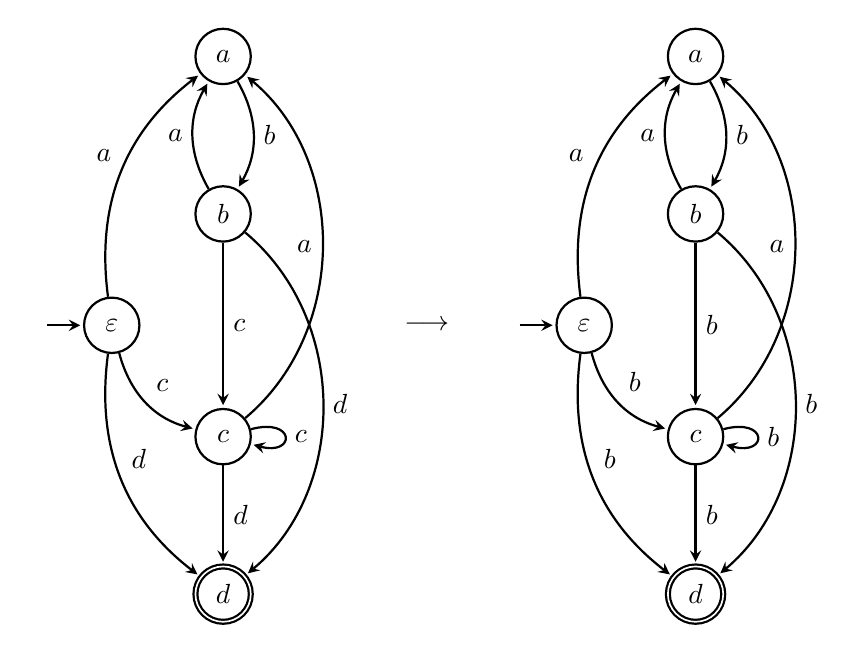
\begin{tikzpicture}[%
    >=stealth,
    shorten >=1pt,
    node distance=2cm,
    on grid,
    auto,
    state/.append style={minimum size=2em},
    thick]
    \node[state, initial, initial text = {}] (epsilon_1) {$\varepsilon$};
    \node[state] (b_1) [above right of=epsilon_1] {$b$};
    \node[state] (a_1) [above of=b_1] {$a$};
    \node[state] (c_1) [below right of=epsilon_1] {$c$};
    \node[state] (d_1) [accepting, below of=c_1] {$d$};

    \node[right= 4 cm of epsilon_1] (lead) {$\longrightarrow$};

    \node[state, initial, initial text = {}, right= 2 cm of lead] (epsilon_2) {$\varepsilon$};
    \node[state] (b_2) [above right of=epsilon_2] {$b$};
    \node[state] (a_2) [above of=b_2] {$a$};
    \node[state] (c_2) [below right of=epsilon_2] {$c$};
    \node[state] (d_2) [accepting, below of=c_2] {$d$};

    \path[->] 
              (epsilon_1) edge [bend left]  node {$a$} (a_1)
              (epsilon_1) edge [bend right] node {$c$} (c_1)
              (epsilon_1) edge [bend right] node {$d$} (d_1)
              (a_1) edge [bend left] node {$b$} (b_1)
              (b_1) edge [bend left] node {$a$} (a_1)
              (b_1) edge [] node {$c$} (c_1)
              (b_1) edge [bend left=50] node {$d$} (d_1)
              (c_1) edge [] node {$d$} (d_1)
              (c_1) edge [loop right] node {$c$} (c_1)
              (c_1) edge [bend right=50] node {$a$} (a_1)
              
              (epsilon_2) edge [bend left]  node {$a$} (a_2)
              (epsilon_2) edge [bend right] node {$b$} (c_2)
              (epsilon_2) edge [bend right] node {$b$} (d_2)
              (a_2) edge [bend left] node {$b$} (b_2)
              (b_2) edge [bend left] node {$a$} (a_2)
              (b_2) edge [] node {$b$} (c_2)
              (b_2) edge [bend left=50] node {$b$} (d_2)
              (c_2) edge [] node {$b$} (d_2)
              (c_2) edge [loop right] node {$b$} (c_2)
              (c_2) edge [bend right=50] node {$a$} (a_2);
  \end{tikzpicture}
\end{document}